%======================================================================
% AI–Powered Knowledge Work – Complete, Spatially Tuned & Photo Included
%======================================================================
\documentclass[aspectratio=169]{beamer}

%---------------------------------------------------------------------
% Theme & Packages
%---------------------------------------------------------------------
\usetheme{CambridgeUS}
\usecolortheme{default}
\usepackage[utf8]{inputenc}
\usepackage{graphicx}
\usepackage{booktabs}
\usepackage{tikz}
\usepackage{fontawesome5}
\usepackage{hyperref}
\usepackage{multicol}
\usepackage{xcolor}

%---------------------------------------------------------------------
% Custom Colours
%---------------------------------------------------------------------
\definecolor{aiblue}{RGB}{79,195,247}
\definecolor{darkblue}{RGB}{1,87,155}
\definecolor{successgreen}{RGB}{76,175,80}
\definecolor{warningorange}{RGB}{255,152,0}
\definecolor{textgray}{gray}{0.15}

%---------------------------------------------------------------------
% Beamer Tweaks
%---------------------------------------------------------------------
\setbeamertemplate{headline}{}
\setbeamertemplate{footline}{}
\setbeamertemplate{navigation symbols}{}
\setbeamercolor{normal text}{fg=textgray,bg=white}
\setbeamercolor{frametitle}{fg=textgray}

%---------------------------------------------------------------------
% Background Helper
%---------------------------------------------------------------------
\newcommand{\UseBackground}[1]{%
  \setbeamertemplate{background}{%
    \begin{tikzpicture}[remember picture,overlay]
      \node at (current page.center) {\includegraphics[width=\paperwidth,height=\paperheight,keepaspectratio]{#1}};
      \fill[white,opacity=0.80] (current page.south west) rectangle (current page.north east);
    \end{tikzpicture}}
}

%---------------------------------------------------------------------
% Document Metadata
%---------------------------------------------------------------------
\title{AI-Powered Knowledge Work}
\subtitle{Master the New Universal Workspace}
\author{Dr. John O'Hare}
\institute{DREAMLAB | Chief Hallucination Officer}
\date{2025}

%=====================================================================
% Document Body
%=====================================================================
\begin{document}

% Slide 1
\UseBackground{slide-1-backdrop.png}
\begin{frame}[plain]\titlepage\end{frame}

% Slide 2
\UseBackground{slide-2-backdrop.png}
\begin{frame}[t]
  \frametitle{The AI Revolution in Knowledge Work}
  \begin{block}{The Paradigm Shift}
    The boundary between \textbf{"technical"} and \textbf{"non-technical"} work has
    \textcolor{aiblue}{\textbf{dissolved}}.
  \end{block}
  \vspace{0.5em}
  \begin{columns}[T,onlytextwidth]
    \column{0.48\textwidth}
      \textbf{Before:}
      \begin{itemize}\itemsep4pt
        \item Copy-paste from ChatGPT
        \item Limited by web interfaces
        \item No version control
        \item Manual repetitive tasks
      \end{itemize}
    \column{0.48\textwidth}
      \textbf{After This Workshop:}
      \begin{itemize}\itemsep4pt
        \item Direct AI API access
        \item VS\,Code as AI command centre
        \item Professional automation
        \item 10× productivity gains
      \end{itemize}
  \end{columns}
\end{frame}

% Slide 3
\UseBackground{slide-3-backdrop.png}
\begin{frame}[t]
  \frametitle{The Professional AI Divide}
  \begin{center}\Large Two Classes of AI Users Are Emerging\end{center}
  \vspace{1em}
  \begin{itemize}\itemsep6pt
    \item \textbf{The 95\%}: Limited to consumer tools, copy-paste workflows
    \item \textbf{The 5\%}: Direct API access, automation, 10× productivity
  \end{itemize}
  \vspace{1em}
  \begin{alertblock}{The Gap Is Widening Daily}
    While most struggle with ChatGPT limits, a small group writes books in days, creates comprehensive documentation in hours, and builds autonomous knowledge systems.
  \end{alertblock}
\end{frame}

% Slide 4
\UseBackground{slide-4-backdrop.png}
\begin{frame}[t]
  \frametitle{Transform Your Professional Practice}
  \begin{columns}[T,onlytextwidth]
    \column{0.45\textwidth}
      \textbf{Perfect For:}
      \begin{itemize}\itemsep4pt
        \item Academics \& Researchers
        \item Business Leaders
        \item Consultants
        \item Government \& NGOs
        \item Creative Professionals
        \item Entrepreneurs
      \end{itemize}
    \column{0.45\textwidth}
      \textbf{If You:}
      \begin{itemize}\itemsep4pt
        \item Work with documents daily
        \item Feel limited by ChatGPT
        \item Need privacy for sensitive data
        \item Want to automate repetitive work
        \item Are curious about AI’s potential
      \end{itemize}
  \end{columns}
  \vspace{0.5em}
  \begin{center}\small{\emph{No coding experience required – if you can use Word, you’re ready}}\end{center}
\end{frame}

% Slide 5
\UseBackground{slide-5-backdrop.png}
\begin{frame}[plain]\end{frame}

% Slide 6
\UseBackground{slide-6-backdrop.png}
\begin{frame}[t]
  \frametitle{Your 5-Day Transformation Journey}
  \begin{center}
    \textbf{From AI Consumer to AI Commander in 5 Days}
  \end{center}
\end{frame}

% Slide 7
\UseBackground{slide-7-backdrop.png}
\begin{frame}[t]
  \frametitle{Programme Structure}
  \footnotesize
  \begin{tabular}{@{}p{0.6cm}p{3.0cm}p{5.5cm}p{3.0cm}@{}}
    \toprule
    \textbf{Day} & \textbf{Theme} & \textbf{Core Focus} & \textbf{Your Win}\\
    \midrule
      1 & \textcolor{aiblue}{Universal Workspace}    & VS\,Code setup, containers, version control     & Professional AI workspace \\
      2 & \textcolor{aiblue}{AI Creative Partner}      & Direct API access, \emph{vibe coding}           & Live website via chat   \\
      3 & \textcolor{aiblue}{Private AI Brain}         & Local models, RAG systems                        & Offline knowledge base  \\
      4 & \textcolor{aiblue}{AI Teams}                & Specialised agents, orchestration                & Automated workflows     \\
      5 & \textcolor{aiblue}{Pro Publishing}          & LaTeX, websites, automation                      & Complete portfolio      \\
    \bottomrule
  \end{tabular}
\end{frame}

% Slides 8–12
% Day 1
\UseBackground{slide-8-backdrop.png}
\begin{frame}[t]
  \frametitle{Day\,1: Your Universal AI Workspace}
  \begin{columns}[T,onlytextwidth]
    \column{0.48\textwidth}
      \textbf{Morning: Setup \& Foundations}
      \begin{itemize}\itemsep4pt
        \item Transform VS Code into AI command centre
        \item Install game-changing extensions
        \item Container setup for stability
        \item Navigate like a pro
      \end{itemize}
    \column{0.48\textwidth}
      \textbf{Afternoon: Visual Tools}
      \begin{itemize}\itemsep4pt
        \item Mermaid diagrams mastery
        \item Version control for \textbf{ANY} document
        \item Build your first repository
        \item Track every change forever
      \end{itemize}
  \end{columns}
  \vspace{0.5em}
  \begin{alertblock}{Day\,1 Deliverable}
    Professional workspace with visual project plan (Gantt chart) for \textbf{YOUR} real project
  \end{alertblock}
\end{frame}

% Day 2
\UseBackground{slide-9-backdrop.png}
\begin{frame}[t]
  \frametitle{Day\,2: AI as Your Creative Partner}
  \begin{block}{The \emph{“Vibe Coding”} Revolution}
    Describe what you want in plain English → AI builds it perfectly
  \end{block}
  \vspace{0.5em}
  \begin{columns}[T,onlytextwidth]
    \column{0.48\textwidth}
      \textbf{Morning: Direct AI Access}\begin{itemize}\itemsep4pt
        \item Connect OpenAI, Claude, Gemini
        \item Compare model strengths
        \item See real API costs (pennies!)
        \item Generate business plans, papers
      \end{itemize}
    \column{0.48\textwidth}
      \textbf{Afternoon: Build by Talking}\begin{itemize}\itemsep4pt
        \item Create websites via chat
        \item Interactive presentations
        \item Data visualisations
        \item Deploy live in minutes
      \end{itemize}
  \end{columns}
  \vspace{0.5em}
  \textcolor{successgreen}{\faCheckCircle} \textbf{Day\,2 Win:} Professional website live on the internet
\end{frame}

% Day 3
\UseBackground{slide-10-backdrop.png}
\begin{frame}[t]
  \frametitle{Day\,3: Your Private AI Brain}
  \begin{alertblock}{Complete Privacy + Total Recall}
    AI that knows your entire document history and works 100\% offline
  \end{alertblock}
  \vspace{0.5em}
  \begin{columns}[T,onlytextwidth]
    \column{0.48\textwidth}
      \textbf{Morning: Local AI Models}\begin{itemize}\itemsep4pt
        \item Install AI on \textbf{YOUR} laptop
        \item No internet required
        \item Perfect for sensitive data
        \item Multiple specialist models
      \end{itemize}
    \column{0.48\textwidth}
      \textbf{Afternoon: RAG System}\begin{itemize}\itemsep4pt
        \item Feed in all your documents
        \item Instant answers with citations
        \item \emph{“What was decided in March?”}
        \item Your personal AI librarian
      \end{itemize}
  \end{columns}
  \vspace{0.5em}
  \begin{center}\small{\emph{Perfect for: Confidential business docs, proprietary research, client data}}\end{center}
\end{frame}

% Day 4
\UseBackground{slide-11-backdrop.png}
\begin{frame}[t]
  \frametitle{Day\,4: AI Teams Working For You}
  \begin{center}\Large Deploy Your AI Workforce\end{center}
  \vspace{0.5em}
  \begin{columns}[T,onlytextwidth]
    \column{0.25\textwidth}\centering
      \faSearch[regular]\quad \textbf{Research Agent}\\ Autonomous research \& fact-checking
    \column{0.25\textwidth}\centering
      \faFile[regular]\quad \textbf{Writer Agent}\\ Creates documents in your style
    \column{0.25\textwidth}\centering
      \faChartBar[regular]\quad \textbf{Analyst Agent}\\ Data processing \& insights
    \column{0.25\textwidth}\centering
      \faRobot[regular]\quad \textbf{Automator}\\ Handles workflows
  \end{columns}
  \vspace{0.5em}
  \begin{block}{Afternoon: Orchestration \& Safety}
    Make agents collaborate • Set spending limits • Quality checks • Cost control
  \end{block}
\end{frame}

% Day 5
\UseBackground{slide-12-backdrop.png}
\begin{frame}[t]
  \frametitle{Day\,5: Professional Publishing Suite}
  \begin{columns}[T,onlytextwidth]
    \column{0.48\textwidth}
      \textbf{Morning: Quality \& Automation}\begin{itemize}\itemsep4pt
        \item Automated quality checks
        \item Weekly report workflows
        \item Safety nets \& approvals
        \item Full system integration
      \end{itemize}
    \column{0.48\textwidth}
      \textbf{Afternoon: Pro Outputs}\begin{itemize}\itemsep4pt
        \item LaTeX academic papers
        \item Interactive business reports
        \item Client microsites
        \item Complete automation
      \end{itemize}
  \end{columns}
  \vspace{0.5em}
  \begin{alertblock}{Final Achievement}
    Complete AI-powered workflow producing professional documents, websites,
    and reports—all connected and automated
  \end{alertblock}
\end{frame}

% Slide 13
\UseBackground{slide-13-backdrop.png}
\begin{frame}[t]
  \frametitle{Real Results from Real Professionals}
  \begin{columns}[T,onlytextwidth]
    \column{0.48\textwidth}
      \begin{block}{Academic Success}
        “Used to spend weeks on grant proposals. Now my AI agents do research, I do strategy.\\ Just won £2M funding.”\\
        \emph{— Dr. Rachel Morrison, Research Director}
      \end{block}
      \vspace{0.5em}
      \begin{block}{Business Transformation}
        “Client reports that took days now take hours, with interactive diagrams.”\\
        \emph{— James Liu, Consultant}
      \end{block}
    \column{0.48\textwidth}
      \begin{block}{Knowledge Management}
        “10 years of company knowledge instantly accessible. Like having our history on tap.”\\
        \emph{— Sandra Patel, Ops Director}
      \end{block}
      \vspace{0.5em}
      \begin{block}{Non-Technical Success}
        “I’m not technical, but built our entire handbook site through conversation.”\\
        \emph{— Michael Chang, HR Director}
      \end{block}
  \end{columns}
\end{frame}

% Slide 14
\UseBackground{slide-14-backdrop.png}
\begin{frame}[t]
  \frametitle{Investment \& Returns}
  \begin{columns}[T,onlytextwidth]
    \column{0.48\textwidth}
      \textbf{Your Investment}\begin{itemize}\itemsep4pt
        \item Standard: £2,995
        \item Early Bird: £2,495 (save £500)
        \item Includes £200 API credits
        \item Payment plans available
        \item Team discounts: 15\% for 3+
      \end{itemize}
    \column{0.48\textwidth}
      \textbf{Documented Returns}\begin{itemize}\itemsep4pt
        \item Grant writing: 70\% faster
        \item Business docs: 5× speed
        \item Research: 10× throughput
        \item ROI in first project
        \item Skills that compound daily
      \end{itemize}
  \end{columns}
  \vspace{0.5em}
  \begin{alertblock}{Satisfaction Guarantee}
    Full refund if not completely satisfied after Day\,1
  \end{alertblock}
\end{frame}

% Slide 15
\UseBackground{slide-15-backdrop.png}
\begin{frame}[t]
  \frametitle{Your Guide: Dr. John O'Hare}
  \begin{columns}[T,onlytextwidth]
    \column{0.45\textwidth}\centering
      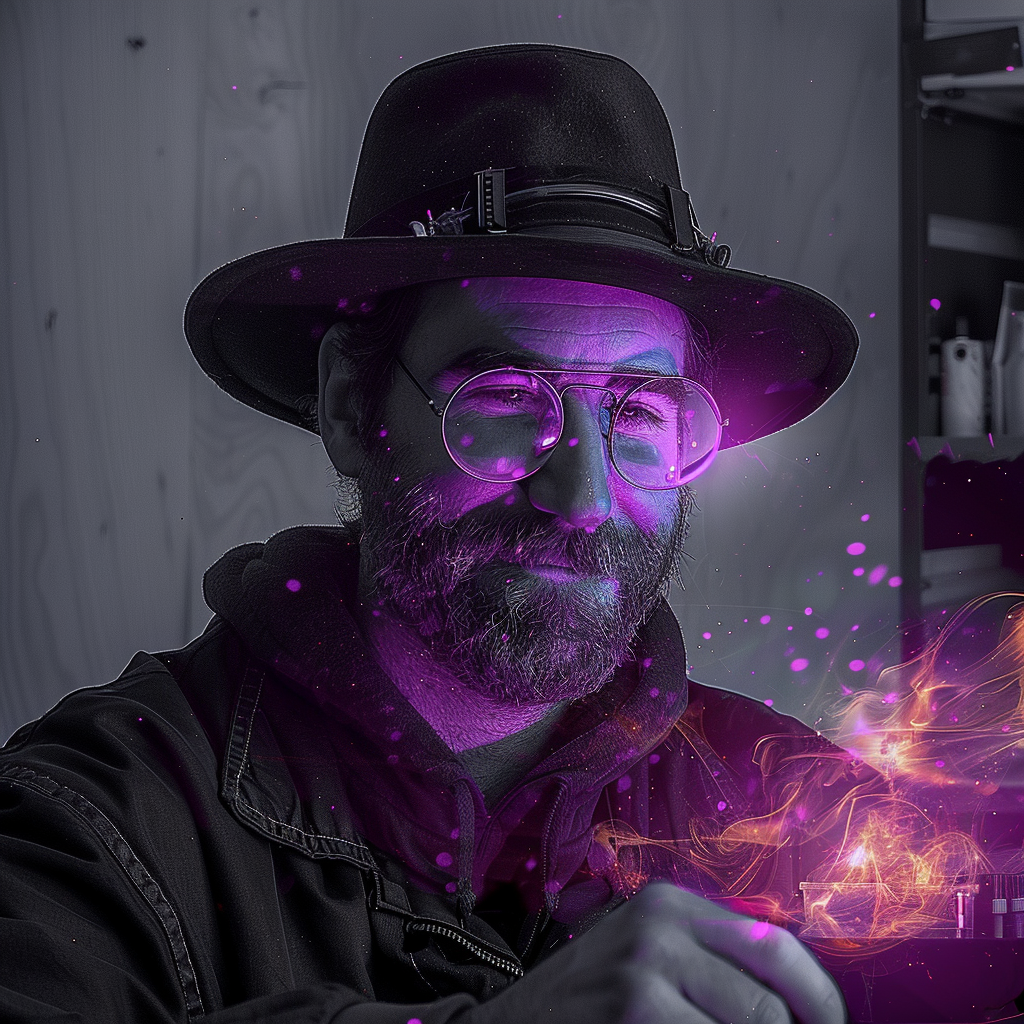
\includegraphics[width=0.6\textwidth]{CHO.png}
    \column{0.55\textwidth}
      \textbf{25+ Years at Tech’s Cutting Edge}\begin{itemize}\itemsep4pt
        \item PhD in collaborative technologies
        \item VR pioneer (1990s) → AI leader (today)
        \item Associate Director R\&D, DREAMLAB
        \item HP AI Lighthouse Partner
        \item Published researcher
        \item 15+ person team leadership
      \end{itemize}
  \end{columns}
  \vspace{0.5em}
  \begin{quote}\small
    “The AI wave is different—faster, more profound, more accessible. This workshop distils decades of experience into skills you can use immediately.”
  \end{quote}
\end{frame}

% Slide 16
\UseBackground{slide-16-backdrop.png}
\begin{frame}[t]
  \frametitle{Why This Workshop Is Unique}
  \begin{columns}[T,onlytextwidth]
    \column{0.48\textwidth}
      \textbf{Our Approach}\begin{itemize}\itemsep4pt
        \item Work on YOUR real projects
        \item Small cohorts (max 10)
        \item Lifetime community access
        \item Quarterly alumni workshops
        \item 30-min mentorship included
      \end{itemize}
    \column{0.48\textwidth}
      \textbf{Unique Features}\begin{itemize}\itemsep4pt
        \item Vendor-agnostic training
        \item Local + cloud options
        \item Privacy-first approach
        \item Cross-industry learning
        \item Immediate application
      \end{itemize}
  \end{columns}
  \vspace{0.5em}
  \begin{block}{Not Just Tools—Transformation}
    Learn principles that remain valuable as AI evolves, not just today’s tools.
  \end{block}
\end{frame}

% Slide 17
\UseBackground{slide-17-backdrop.png}
\begin{frame}[t]
  \frametitle{Secure Your Transformation}
  \begin{alertblock}{Next Cohorts – Limited to 10 Participants}
    \begin{itemize}\itemsep4pt
      \item \textbf{March 2025}: 17–21 March (3 seats remaining)
      \item \textbf{May 2025}:   12–16 May (Early bird available)
      \item \textbf{July 2025}:  14–18 July (Just announced)
    \end{itemize}
  \end{alertblock}
  \vspace{0.5em}
  \textbf{How to Join:}\begin{enumerate}\itemsep4pt
    \item Complete online application (5 minutes)
    \item Brief screening call (15 minutes)
    \item Secure with £500 deposit
    \item Receive pre-course materials
    \item Join cohort Discord
  \end{enumerate}
  \vspace{0.5em}
  \begin{center}\Large\textcolor{aiblue}{\textbf{workshops@dreamlab.uk}}\\
    \small Stop using AI like everyone else. Start commanding it like the few who know how.
  \end{center}
\end{frame}

% Slide 18
\UseBackground{slide-18-backdrop.png}
\begin{frame}[plain]
  \vfill
  \centering
    {\Huge \textbf{The Choice Is Yours}}\\[1em]
    Remain limited by consumer AI tools…\\[0.8em]
    {\Large \textbf{OR}}\\[0.8em]
    {\Large \textcolor{aiblue}{Gain professional-grade control that transforms how you work}}\\[2em]
    {\LARGE workshops@dreamlab.uk}
  \vfill
\end{frame}

\end{document}
